\documentclass[a4paper,12pt]{article}

\usepackage[margin=2cm]{geometry}
\usepackage{graphicx}
\usepackage{amsmath}
\usepackage{array}
\usepackage{hyperref}
\usepackage[all]{hypcap}
\usepackage{listings}
\lstdefinestyle{TerminalStyle}{
  language=bash,
  basicstyle=\small\sffamily,
  numbers=left,
  numberstyle=\tiny,
  numbersep=3pt,
  frame=tb,
  columns=fullflexible,
  linewidth=0.9\linewidth,
  xleftmargin=0.1\linewidth
}
\lstdefinestyle{HtmlStyle}{
  language=html,
  basicstyle=\small\sffamily,
  numbers=left,
  numberstyle=\tiny,
  numbersep=3pt,
  frame=tb,
  columns=fullflexible,
  linewidth=0.9\linewidth,
  xleftmargin=0.1\linewidth
}
\lstdefinestyle{OutputStyle}{
  language=html,
  basicstyle=\small\sffamily,
  frame=tb,
  columns=fullflexible,
  linewidth=0.9\linewidth,
  xleftmargin=0.1\linewidth
}

\setlength{\parindent}{0pt}
\setlength{\parskip}{1ex plus 0.5ex minus 0.2ex}

\title{
\includegraphics[width=12cm]{Eeufeeslogo.jpg} \\
       Department of Computer Science \\
       University of Pretoria \\
       \vspace{0.5cm}
       COS730 Software Engineering \\
       \vspace{0.5cm}
       \begin{large} \textbf{Software Requirement Specifications}\end{large}}

\date{07 March 2018} 
\author{	JM Bondjobo		13232852 \\
		Martha Mohlala		10353403\\
		D Jansen van Vuuren	18364412\\
		 KJ Muranga         13278012        \\
		 RT Mabaso          18296272 \\
         F van der Merwe 18358137
}

\begin{document}
\maketitle
\thispagestyle{empty}
\clearpage

\newpage
\pagenumbering{roman}
\thispagestyle{empty}
\tableofcontents
\clearpage

\newpage
\pagenumbering{arabic}

\section {Introduction}
This section gives a scope description of the benchmark service system. Also, the purpose for this document is described and a list of abbreviations and definitions is provided.
\subsection{Purpose}
The goal of this document is to give a detailed description of the  benchmarking service. It will explain the purpose and features of the system, the interfaces of the system, what the system will do and the constraints under which it must operate.


\subsection{Scope}
The benchmarking service will accept a user's source code and measure its performance in terms of CPU time, elapsed time, memory usage, power consumption, temperature, and other metrics. The user's source code could be either an algorithm or a data structure, and the system should give the user a choice of which programming languages their source code can be implemented in. The service should be provided by executing the requested benchmarks on isolated machines where the side-effects that are not a concern of the specified benchmark are minimized.

The system will be used as an integral part of research related to the development of new algorithms and techniques as well as the refinement and optimization of existing operations. It can also be used to as a teaching tool for students to review the notions of space and time complexity.



\subsection{Definitions, Acronyms and Abbreviations}
\begin{center}
\begin{tabular}{ |p{5cm}|p{10cm}| } 
\hline
Term & Definition \\ 
\hline
User & Individual who uses the benchmarking system. \\ 
\hline
Software Requirements Specification & A document that completely describes all of the functions of a proposed system and the constraints under which it must operate. For example, this document. \\ 
\hline
Benchmark & Evaluate (something) by comparison with a standard. \\
\hline
RAM & Random Access Memory  \\
\hline
HTTP & HyperText Transfer Protocol \\
\hline
TCP & Transmission Control Protocol\\
\hline
\end{tabular}
\end{center}

\subsection{References}
IEEE. IEEE Std 830-1998 IEEE Recommended Practice for Software Requirements Specifications. IEEE Computer Society, 1998

\subsection{Overview}
The remainder of this document consists of two chapters. In the second chapter you will find the Overall Description section which gives a description of the system's functionality. It describes the informal requirements and is used to establish a context for the technical requirements specification in the next chapter.

In the third chapter you will find the Specific Requirements section which gives a detailed description of the benchmarking service. It describes in technical terms the details of the functionality of the system.

\section{Overall Description}
\subsection{Product Perspective}

\subsubsection{System Interfaces}
The system will provide a web interface for users to request and specify the benchmarking services they need. The system interface is depicted as below:\\
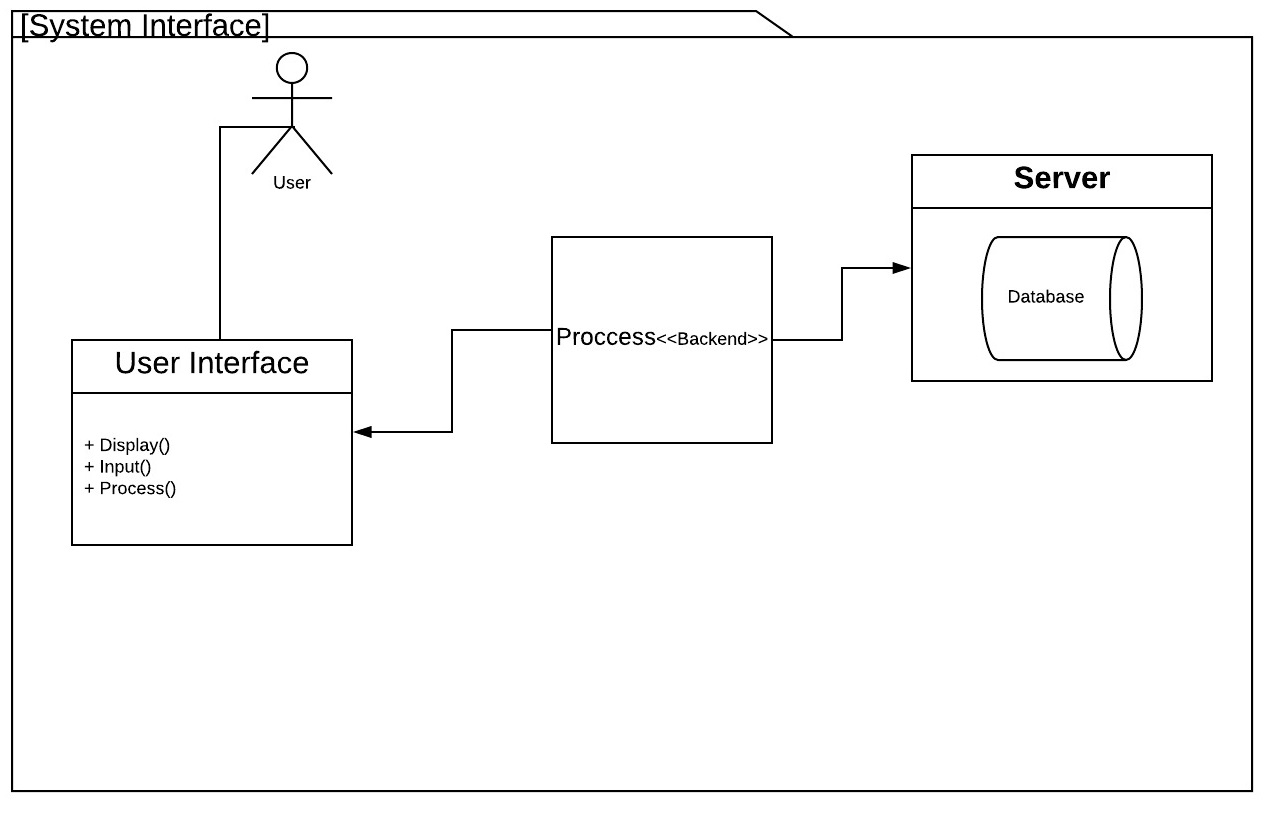
\includegraphics[width=12cm]{SI.jpeg}
\subsubsection{User Interfaces}
The system will have a user interface where the user will interact with the system by inputing variables as well as an executable program and getting statistics about the execution of said program as a response. This is the front-end part of the system that the user will be interacting with. The benchmark tool will follow basic Windows style and functionality conventions. The interface will have a menu where the user will be able to input their variables as well as to add source code that will be executed, a log button on the menu to see what services were done on the computer and by who, a section where the user can track progression of the execution and retrieve any notifications pushed by the benchmark tool and a quick access button to terminate the benchmarking process if the user choose so. 
\subsubsection{Hardware Interfaces}
The system will run on a computer that has at least 100 MB of free space on the hard drive and 1 GB of Ram. The computer used must be an isolated machine where the benchmarking service will be done in order to reduce/ minimize the side effects of others programs running simultaneously. The system does not write information directly to the user's computer. But instead uses a database which is located on a network server. The user's computer transfers and receives data using basic networking protocols like HTTP. All systems' information is stored in the server's database which stores the data on the server's disk reason being if the system runs out of memory or fails during benchmarking the previously gathered information remains on the server's database.
\subsubsection{Software Interfaces}
The system requires a properly configured version of Windows 7 or later to run the application. The system's server can either be Windows or Linux but must have a MySQL database properly installed and configured. The software interface will be web based, therefore must have Microsoft .NET Framework 1.1 or greater installed and for the designing of the benchmarking that can be done using Adobe XD.

\subsubsection{Communication Interfaces}
The benchmarking system will have a network server that is web-based. The server exists to retrieve information from the database
and compute the services in terms of the benchmark metrics provided. The web interface will also query the database for the historical computations of the benchmark metrics. The HTTP server will be used to send the requests from the web interface to the benchmarking system. The web application will support most popular browsers such as but not limited to Chrome, Firefox and Safari.
\subsubsection{Memory}
The system will not use memory less than 100 MB of the hard drive and 1 GB of RAM as described on the hardware interface.
\subsubsection{Operations}
The user will initiate the request for benchmarking services and wait for response. The response might take a while as the system is required to do computation and comparison between two inputs. The user will have an option of inputting algorithms or data structures and the input will be validated to check if it is algorithm or data structure. The system will also allow the user to store all the computation and comparison results to the database as historical data to avoid computing the same request many times, and also for recovery. 
\subsubsection{Site Adaptation Requirements}
The program or tool must be able to view code. It must measure CPU (Central Processing Unit) performance, memory usage (RAM), temperature, power consumption and other metrics.
It should also ideally be able to accept and handle any modern coding languages such as Java, C\#, C++ etc. The program must also be a web-application that can compile code and test for its runtime attributes. 
The user must select their programming language and then input the code. The program then compiles the code and give feedback on power usage, temperature difference etc. This will all be done in a web-application.

\subsection{Product Functions}
The software will perform a list of functions like:
\begin{itemize}
\item Check what language the code is written in.
\item Minimize main application concern
\item Calculate memory usage
\item Calculate temperature difference
\item Calculate power consumption
\item Calculate CPU usage
\item Give feedback.
\end{itemize}
	
These functions must be executed and the correct feedback must be given. For instance, when the user's code is compiled, the calculation must not measure performance changes to the program, but rather only to the user's code. 
The process of the functions are as follows:
\begin{itemize}
\item User selects programming language
\item User inputs their code.
\item Measure performance and hold information
\item Handle any exceptions that might occur
\item Give performance feedback
\end{itemize}



\subsection{User Characteristics}
An average user does not even need to have a programming background. If the user needs to test the performance of code and give the feedback back to the developer, they can. They can simply copy the code into the program and get the results. One of the goals of the application is to give feedback in a very user friendly manner, this will allow any user to use this web-application without any development background

Graphs can be created to give users an even better understanding of how the application measures performance. 

\subsection{Constraints}
Limitations to developer options can include the following:
\begin{itemize}
\item Programming knowledge (Being able to only compile code that the developers know of).
\item Parallel operation (Measuring one program inside another program).
\item Control function (Test whether user code will "break" our program).
\item If user's device is to slow (Hinder measuring process may result in inaccurate results).
\end{itemize}

\subsection{Assumptions and Dependencies}
To reach this benchmark tool online it is assumed that the tool might be deployed to an off site computer such as the cloud. A possible solution would be AWS, Amazon's cloud based solution. Dependencies includes but are not limited to JDK 1.8 and Oracle drivers as well as an inbound and outbound network rules to allow users to communicate with the program and also to allow the program to connect to external resources. There will also be an dependency toward an Oracle database as this would be where sample data is stored. The application would also need a container such as Weblogic to preside in. This would make it easier to not only gain access to the benchmark tool but also to obtain the necessary statistics to display to the user. 

\section{Specific Requirements}

\subsection{External Interface Requirements}
The system that needs to be developed is a coding benchmarking tool. The system shall perform a benchmark on executable code the user inputs. The benchmark will obtain data from an Oracle database execute the code and then return statistics about the resources the code used when it was executed.
Hardware interface
Input
\begin{itemize}
\item The amount of memory made available to execute the code.
\item The amount of CPU cores made available to execute the code. 
\item The amount of threads the application is allowed to use.
\end{itemize}
Output
\begin{itemize}
\item The CPU usage that the program used while executing excluding the usage the benchmarking tool itself
\item The temperature levels the CPU reached while executing the user's program. It would be in a Celsius and Fahrenheit format
\item The amount of CPU cores used to execute the program.
\item The name of the CPU that is used to execute the program. 
\item The amount of threads that might have been used to execute the program excluding the usage the benchmarking tool itself. 
\item The amount of memory the program used while executed excluding the usage the benchmarking tool itself. The format would be in byte format such as MB or KB
\item The amount of memory that was made available for the program to be executed. The format would be in byte format such as MB or KB
\end{itemize}
Software interface
Input:
\begin{itemize}
\item The code the user wants to execute.
\item The language type the user wants to execute.
\item Any external  sample data (if applicable) that is needed to execute the program.
\item A time limit (if any) to execute the program
\end{itemize}
Output
\begin{itemize}
\item Will show statistics about the hardware usage as specified above. The statistics might be presented in different ways such as graphs or through the use of progress bars. 
\item The software should also show any relevant statistics that the network used. 
\item If the program was executed previously, this statistics would be used to also compare previous performances the program achieved on that benchmark
\item The overall time used to execute the program would be displayed.
\item If there are any sub sections to the code that is used while executing this would be timed on its owned and also displayed.
\item The time it took to make any external connections and the time it kept the connections open would also be displayed.  
\end{itemize}
Communication Interface
Input:
\begin{itemize}
\item A TCP connection to any external resource the program might need to achieve its goal (A connection to an external database or a container such as Weblogic) 
\item Local connections to any resources needed such as retrieving local test data from Oracle
\end{itemize}
Output:
\begin{itemize}
\item The network usage if the program made any external connections. The format would be in a byte formate accumulated over time such as GB, MB or KB.
\item The average speed the network used toward the external resource as well as the top speed it reached. The format of this usage would possible be in byte per second format such as GB/s, MB/s or KB/s 
\item The local connection usage the program used. The format would be in a byte formate accumulated over time such as GB, MB or KB.
\item The average speed local connections used as well as the top speed. The format of this usage would possible be in byte per second format such as GB/s, MB/s or KB/s 
\end{itemize}


\subsection{Functional Requirements}
 The system will provide the user an interface to execute an application of their choosing. Input checks would include to see if the format of the input is correct such as number only input blocks, code format and time format. Whether the language specified is valid and the code adheres to the specified language's format so that the benchmark tool would be able to know how to execute the program. 
 
 The requirements to follow are:
\begin{enumerate}
\item The benchmark tool must validate any input given by the user
\item A connection to the local database would be made
\item The benchmark tool must start executing after request initiation
\item During execution the benchmark tool must accumulate the necessary statistics that would display in the output
\item Also if there are any external connections made by the application. It must be done so during execution. 
\item Any limits must be kept in mind and if the program surpasses the limit specified the user must be notified but execution should continue if possible.
\item  If the program throws an exception but it did not lead the program to crash the benchmark tool must notify the user and continue execution.
\item If a situation occurred while the program was executed all relevant statistics should be displayed as well as the problem that lead to why execution was not successful
\item If no unforeseen situations occurred and the program executed successfully, the statistics should be displayed
\item The statistics should be logged and stored in the database. This is to record history and to allow the user to gain access to it at a later stage.
\end{enumerate}

Abnormal situations that might occur are:
\begin{itemize}
\item Not obtaining a connection to the local database. 
\item An exception thrown by the benchmark tool. In cases such as
\begin{itemize}
\item Not being able to execute the program for unknown reasons 
\item Unable to obtain statistics while performing the execution operation
\item Unable to obtain any external connections the program wanted to create
\item The program crashed 
\item An internal exception occurred in the benchmark tool itself
\end{itemize}
\item If the program takes to long to progress an timeout exception should be thrown. This is to avoid dead locks or unending loops.
 
\end{itemize}
Most input output relationships are centered around the software interface as the software interface communicates with the network interface and hardware interface to accumulate the statistics needed to present after execution. 

\subsection{Performance Requirements}
While the program is executed, the system should keep track of its progression. If the program that is being executed gets stuck say in a endless loop or a deadlock, an timeout exception would be thrown and the user would be notified.
If the system loses connection to the internet, an error message will display on the user's browser, notifying the user connection has been lost but the execution on the system will continue, store the statistics obtained after the execution so that when the user has regained internet connection they will be able to obtain the statistics stored. 
\subsection{Design Constraints}
The system would only be able to allow a certain amount of users to execute their programs synchronously since the hardware is limited. The problem faced is that if the two users execute their programs asynchronously one users program might dominate the other's program and use all the memory made available. This would lead to inaccurate statistics.  The aim is to get the most accurate statistics, running multiples users programs at the same time might compromise this. 
\subsection{Software System Attributes}
\subsubsection{Reliability}
The system should work reliably, with automatic backup and recovery features. In case of unexpected operating system error or shut-down. The system will be able to save all the computation and comparison results to the database. If the user's program throws an exception and is able to continue executing the user will be notified and the system will continue executing. If the program crashes statistics accumulated up to that point will be displayed as well as the exception that occur during the crash. It does not matter if there is a constant internet connection from the user to the system as all the system needs is the input. After the input is given all operations works off site and also the statistics are stored in a database off site. The user can check back any time on the results the benchmark tool reproduced. This will save head aches from the user's side as well as the system side.
\subsubsection{Availability}
The system will be deployed to a cloud base solution. This will allow availability at any time of the day. The only limitation the system might run into is multiple users want to use the system at the same time. A queue solution would be used to execute the program of the different users.
\subsubsection{ Security }
The system should be access only by the registered users, users could be authenticated by Kerberos or a LDAP solution. Security would be implemented inside the benchmark tool it self as the code that is given by the user might exploit the system. Also trusted sources as external resources may be used by the program but any unknown third party resources should not be allowed.   
\subsubsection{Maintainability}
All code for the benchmark tool shall be well documented as this would help future developers or current developers to easily find a bug and or add a feature if need be. Server side logging should also be incorporated, to catch any exceptions that might be thrown by the tool. A notification system should be put in place to notify the client or developers if the benchmark tool went down.
\subsubsection{Portability}
Gaining access to the benchmark tool should be fairly simple as it is a web app. Most popular browsers should be able to access it from any OS. As far as portability goes at the back end, an image of each release version would be kept. This is to roll back any changes made that have put the system in an unpredictable state. Keeping an image not only maintain a copy of stable state but also to deploy it easily to any other computer solution if so need be. 
\subsubsection{Usability}
 The GUI should be very user friendly. This could be achieved by labeling most of the input boxes and also to show warning messages if the user did not input the correct format. Notifications would also be used to keep the user up to date as to what the current state is. Doing so would make it easy for a user with or without any programming history. A simple tutorial system should also be put in place for the user to use if they might find them self lost.

\newpage
\clearpage
\addcontentsline{toc}{section}{References}

\end{document}
